{\begin{abstract}
本節では,PolylibおよびMPIPolylibの内部設計について,UMLシーケンス図を用いて説明します.
\end{abstract}
%

\graphicspath{{./fig_design/}}

%
\section{Polylibクラス}

%
\subsection{Polylib::load()の内部処理シーケンス}

\begin{figure}[H]
 \centering
 \includegraphics[width=16cm]{clip012.eps}
\end{figure}


\pagebreak
%
\subsection{Polylib::search\_polygons()の内部処理シーケンス}

\begin{figure}[H]
 \centering
 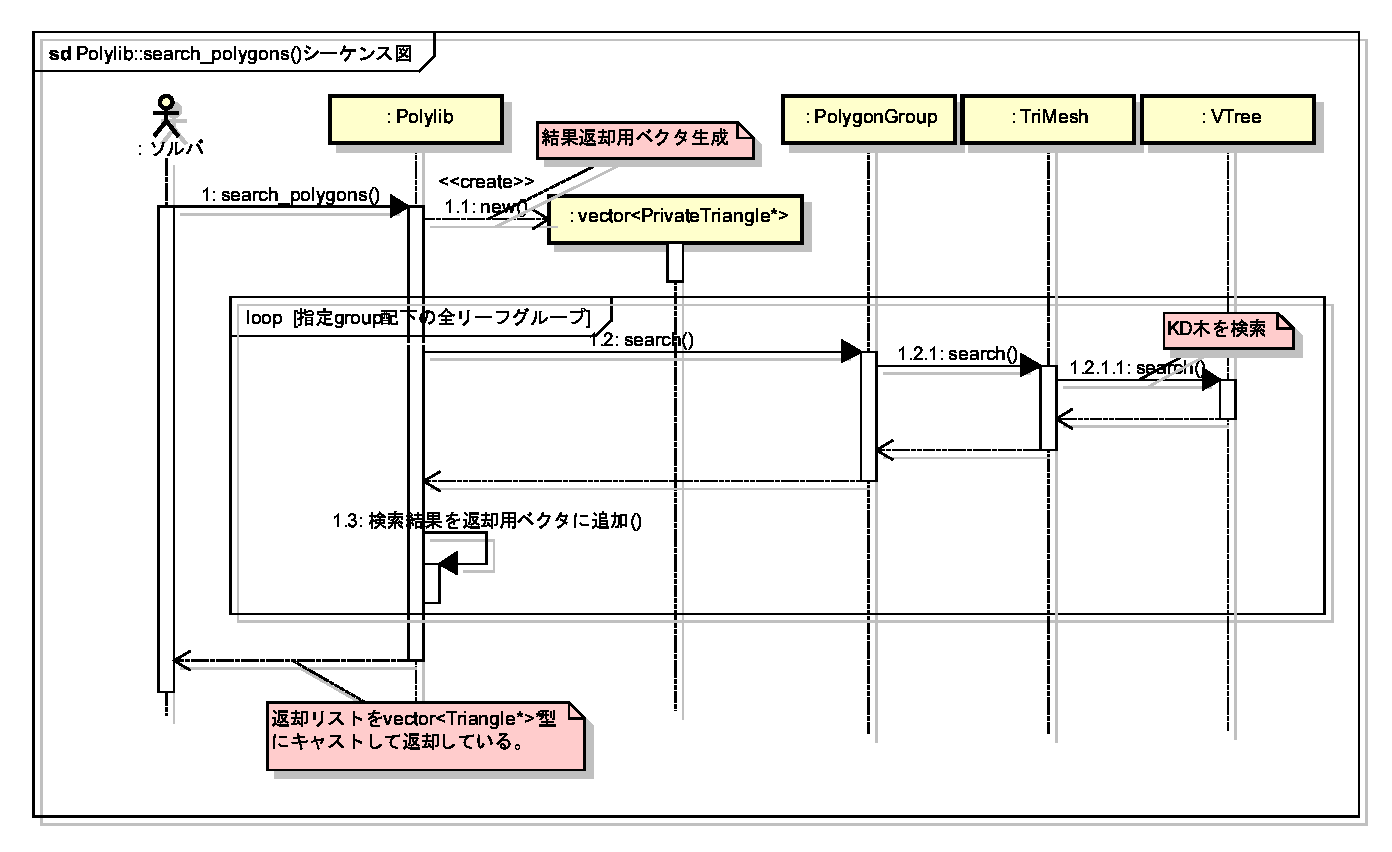
\includegraphics[width=15cm]{clip013.eps}
\end{figure}


%
\subsection{Polylib::move()の内部処理シーケンス}

\begin{figure}[H]
 \centering
 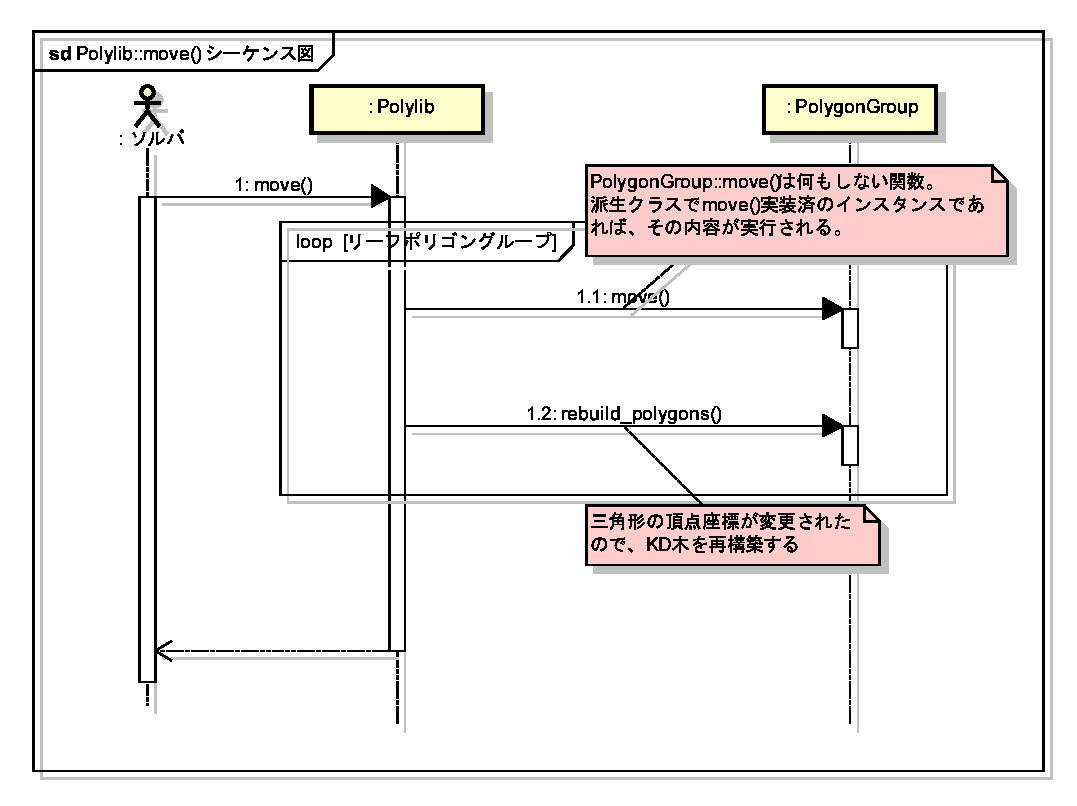
\includegraphics[width=12cm]{clip014.eps}
\end{figure}


\pagebreak
%
\subsection{Polylib::save()の内部処理シーケンス}

\begin{figure}[H]
 \centering
 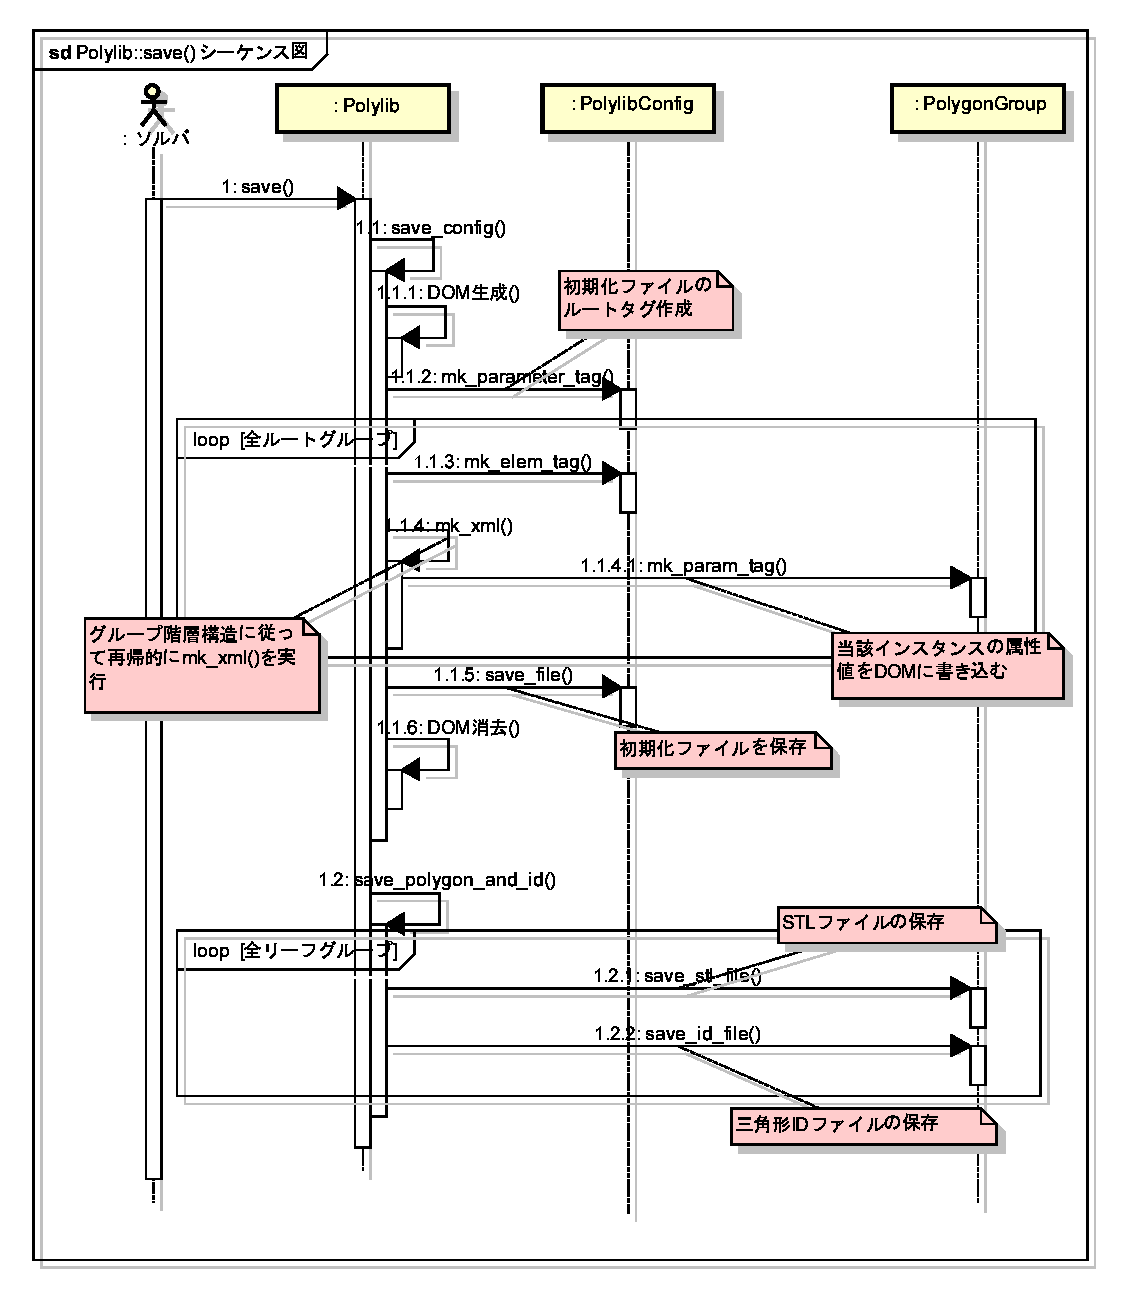
\includegraphics[width=15cm]{clip015.eps}
\end{figure}


\pagebreak
%
\section{MPIPolylibクラス}

%
\subsection{MPIPolylib::init\_parallel\_info()の内部処理シーケンス}

\begin{figure}[H]
 \centering
 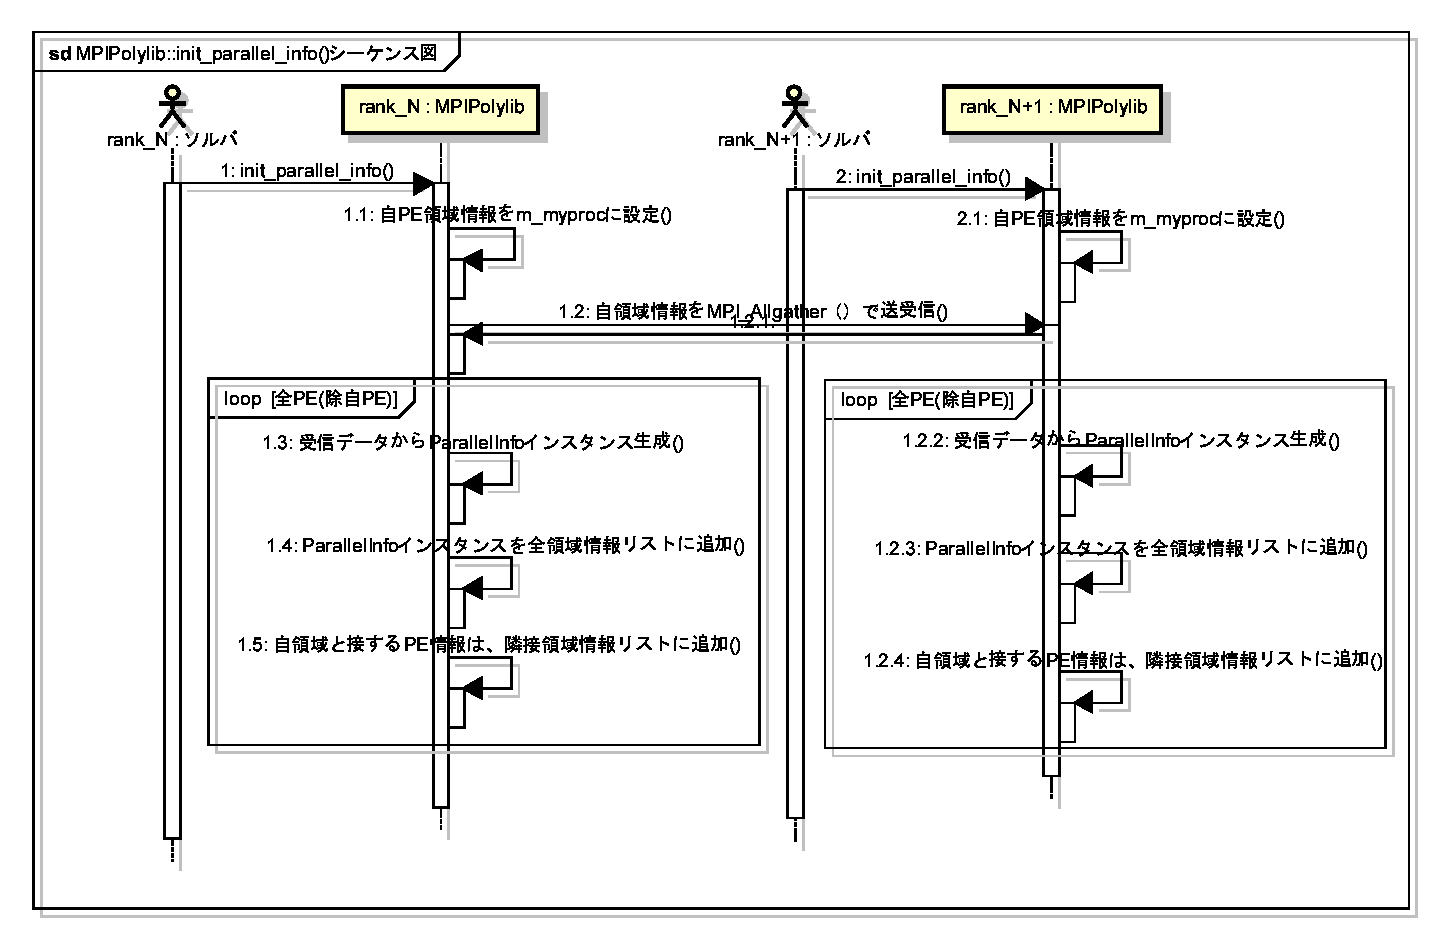
\includegraphics[width=16cm]{clip016.eps}
\end{figure}


\pagebreak
%
\subsection{MPIPolylib::load\_rank0()の内部処理シーケンス}

\begin{figure}[H]
 \centering
 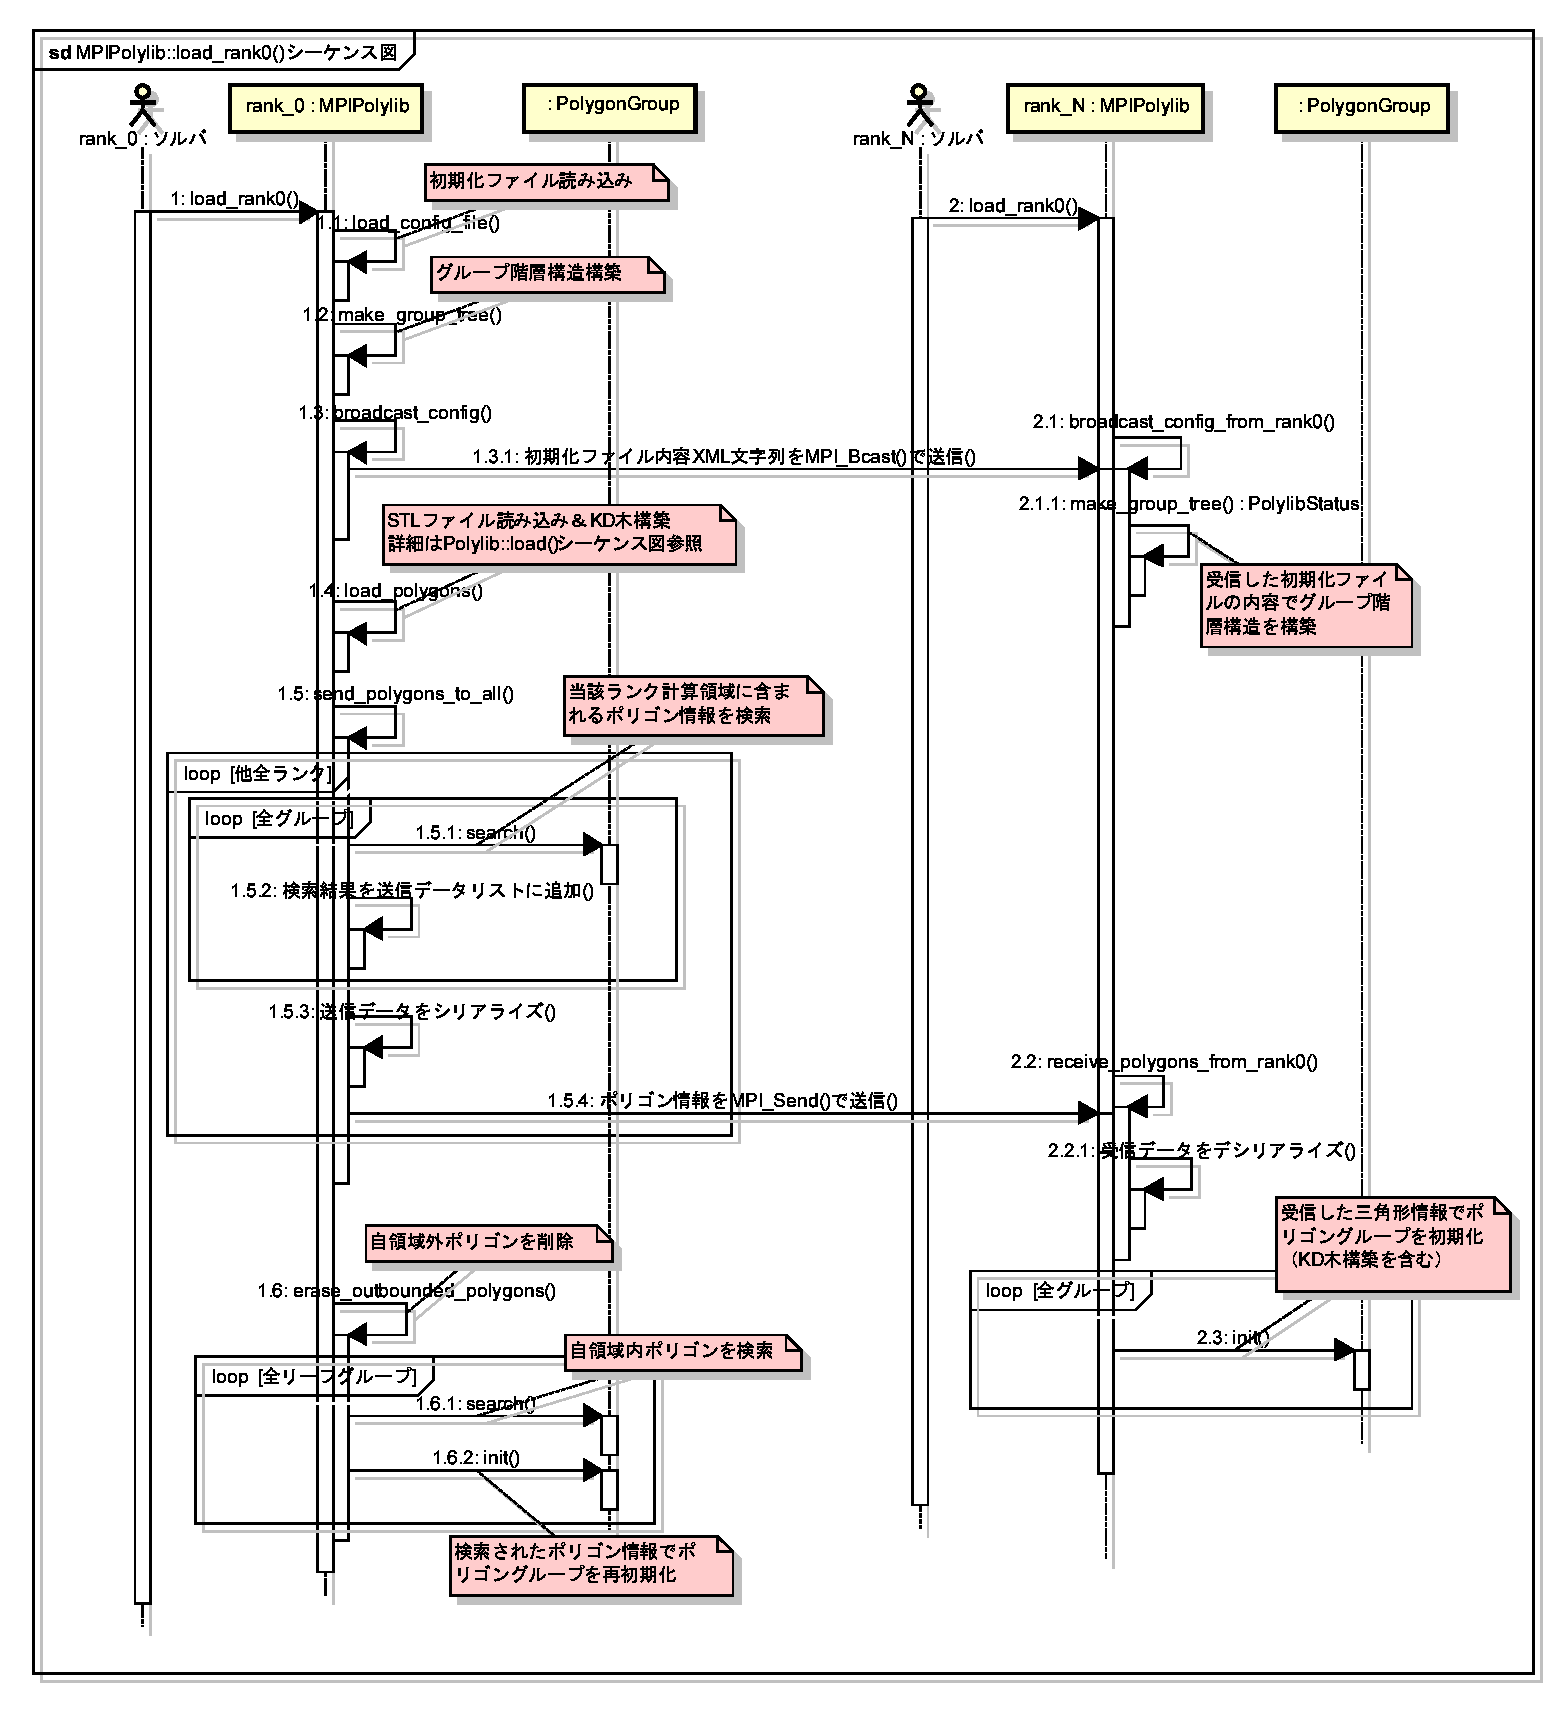
\includegraphics[width=16cm]{clip017.eps}
\end{figure}


\pagebreak
%
\subsection{MPIPolylib::load\_parallel()の内部処理シーケンス}

\begin{figure}[H]
 \centering
 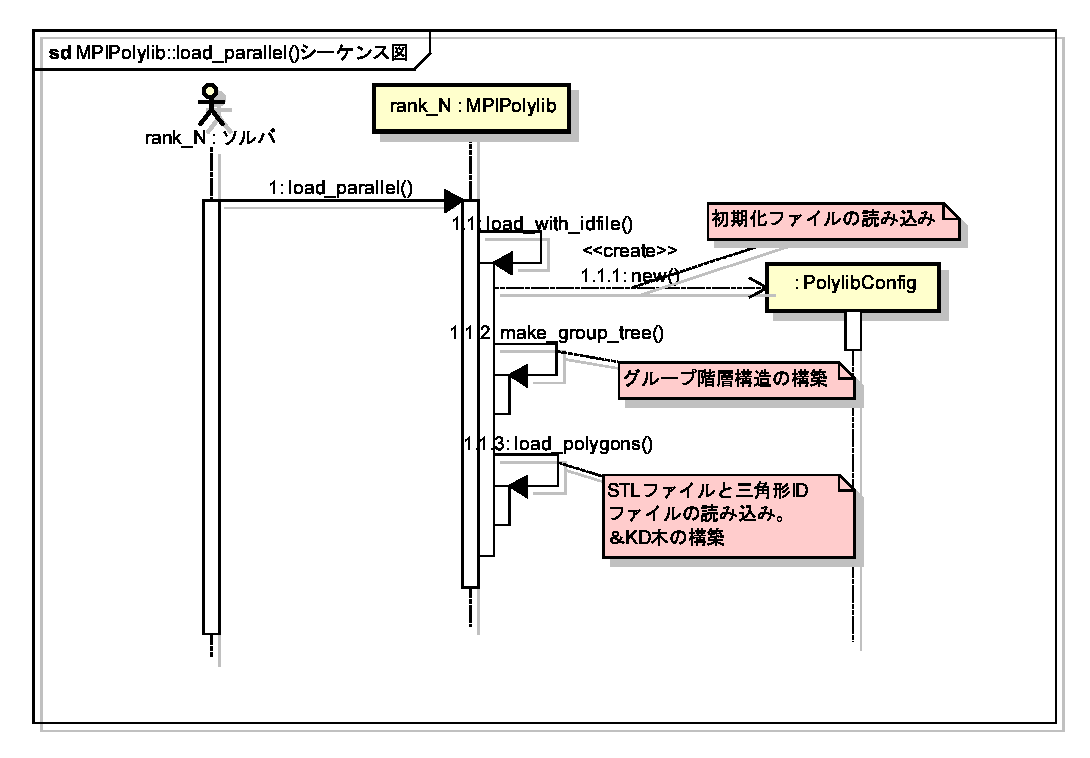
\includegraphics[width=13cm]{clip018.eps}
\end{figure}

%
\subsection{MPIPolylib::move()の内部処理シーケンス}

\begin{figure}[H]
 \centering
 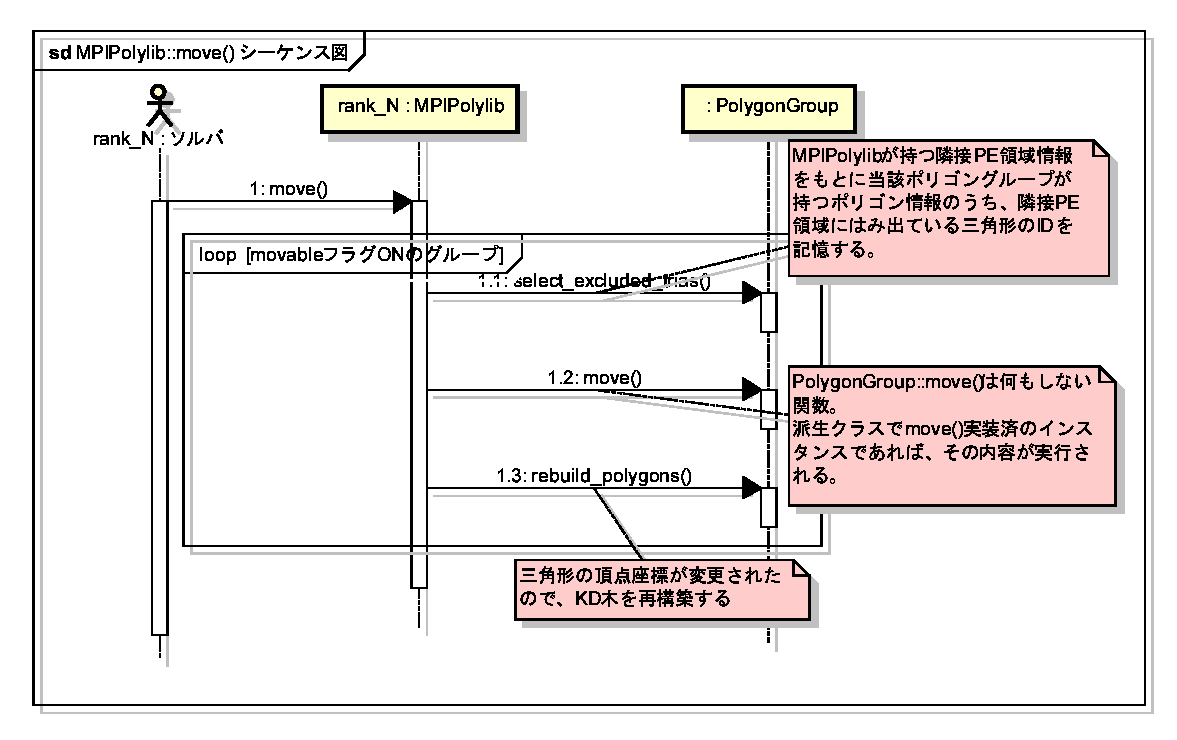
\includegraphics[width=13cm]{clip019.eps}
\end{figure}


\pagebreak
%
\subsection{MPIPolylib::migrate()の内部処理シーケンス}

\begin{figure}[H]
 \centering
 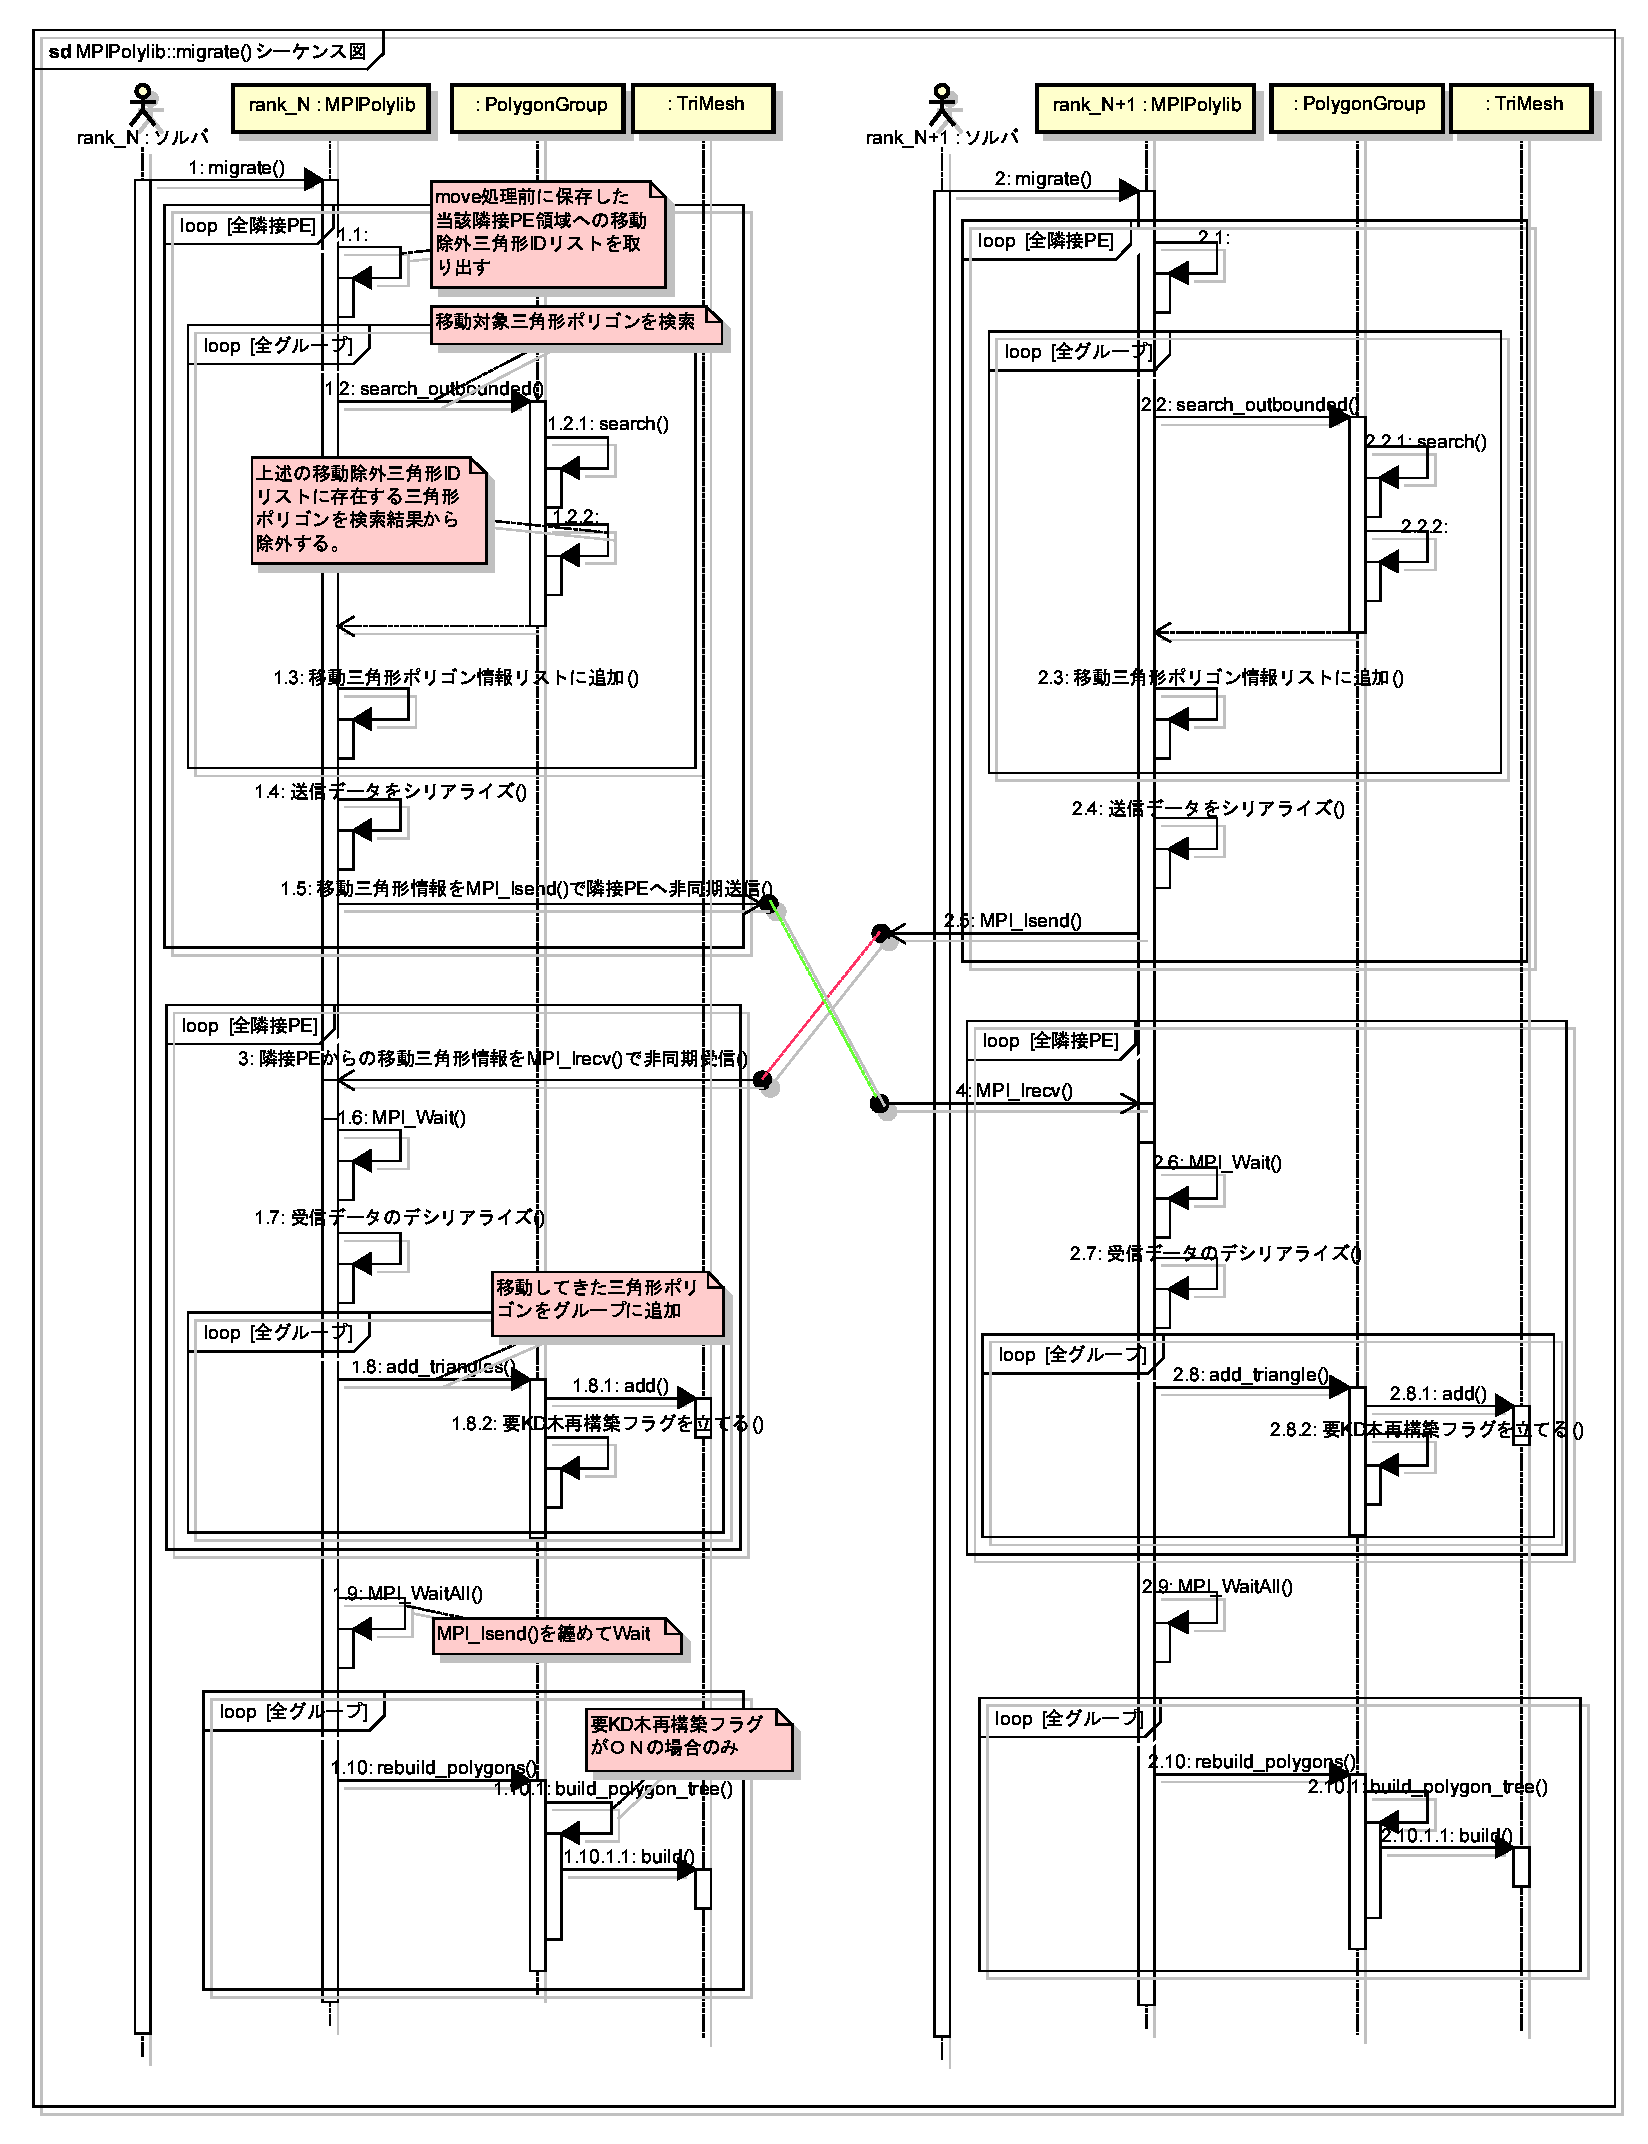
\includegraphics[width=16cm]{clip020.eps}
\end{figure}


\pagebreak
%
\subsection{MPIPolylib::save\_rank0()の内部処理シーケンス}

\begin{figure}[H]
 \centering
 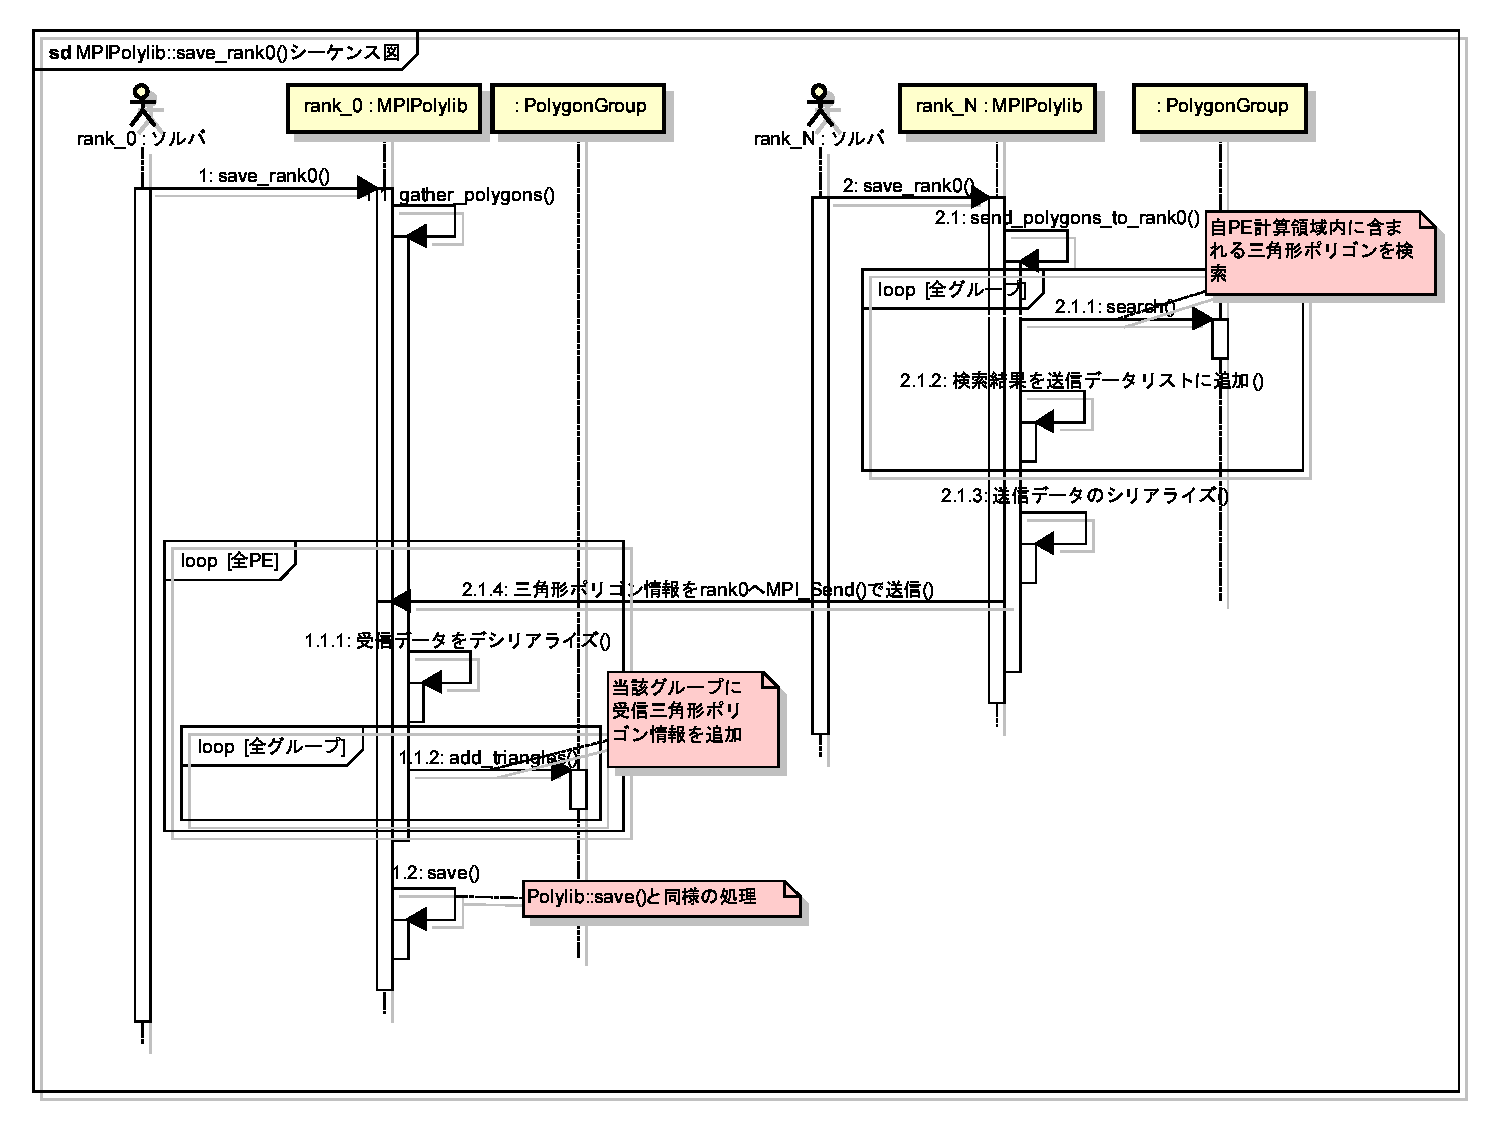
\includegraphics[width=16cm]{clip021.eps}
\end{figure}


\pagebreak
%
\subsection{MPIPolylib::save\_parallel()の内部処理シーケンス}

\begin{figure}[H]
 \centering
 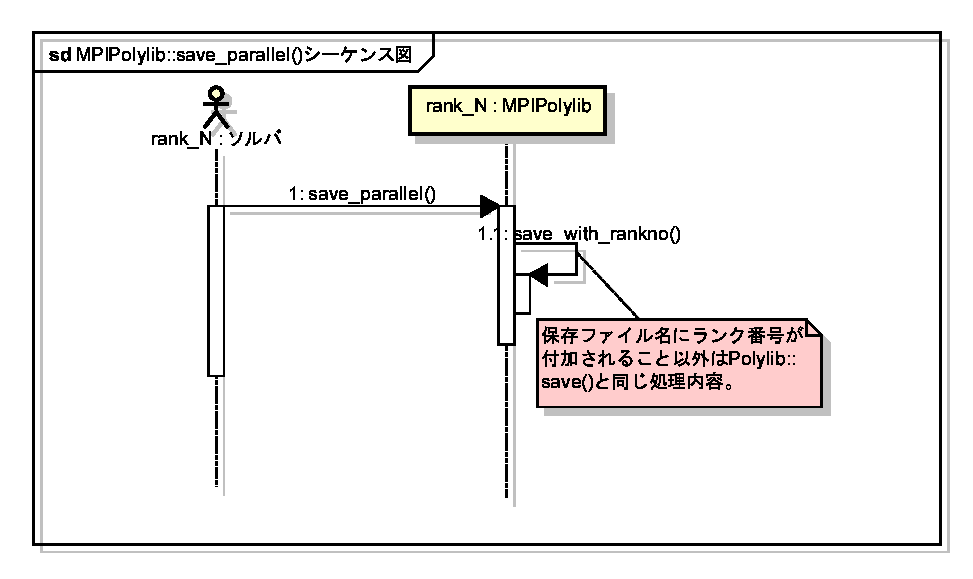
\includegraphics[width=12cm]{clip022.eps}
\end{figure}


\pagebreak
%
\subsection{(参考)MPIPolylibにおけるポリゴンの動的登録に関する検討結果}

Polylib Ver.2.0では,動的なポリゴングループの追加や削除に対応していません.これは開発時点
でその必要性について検討段階であったためです.

以下UMLシーケンス図はソルバー実行中にVOFLibにより新たにポリゴン情報が生成され,それを
MPIPolylibに登録した際の内部処理案です.

\begin{figure}[H]
 \centering
 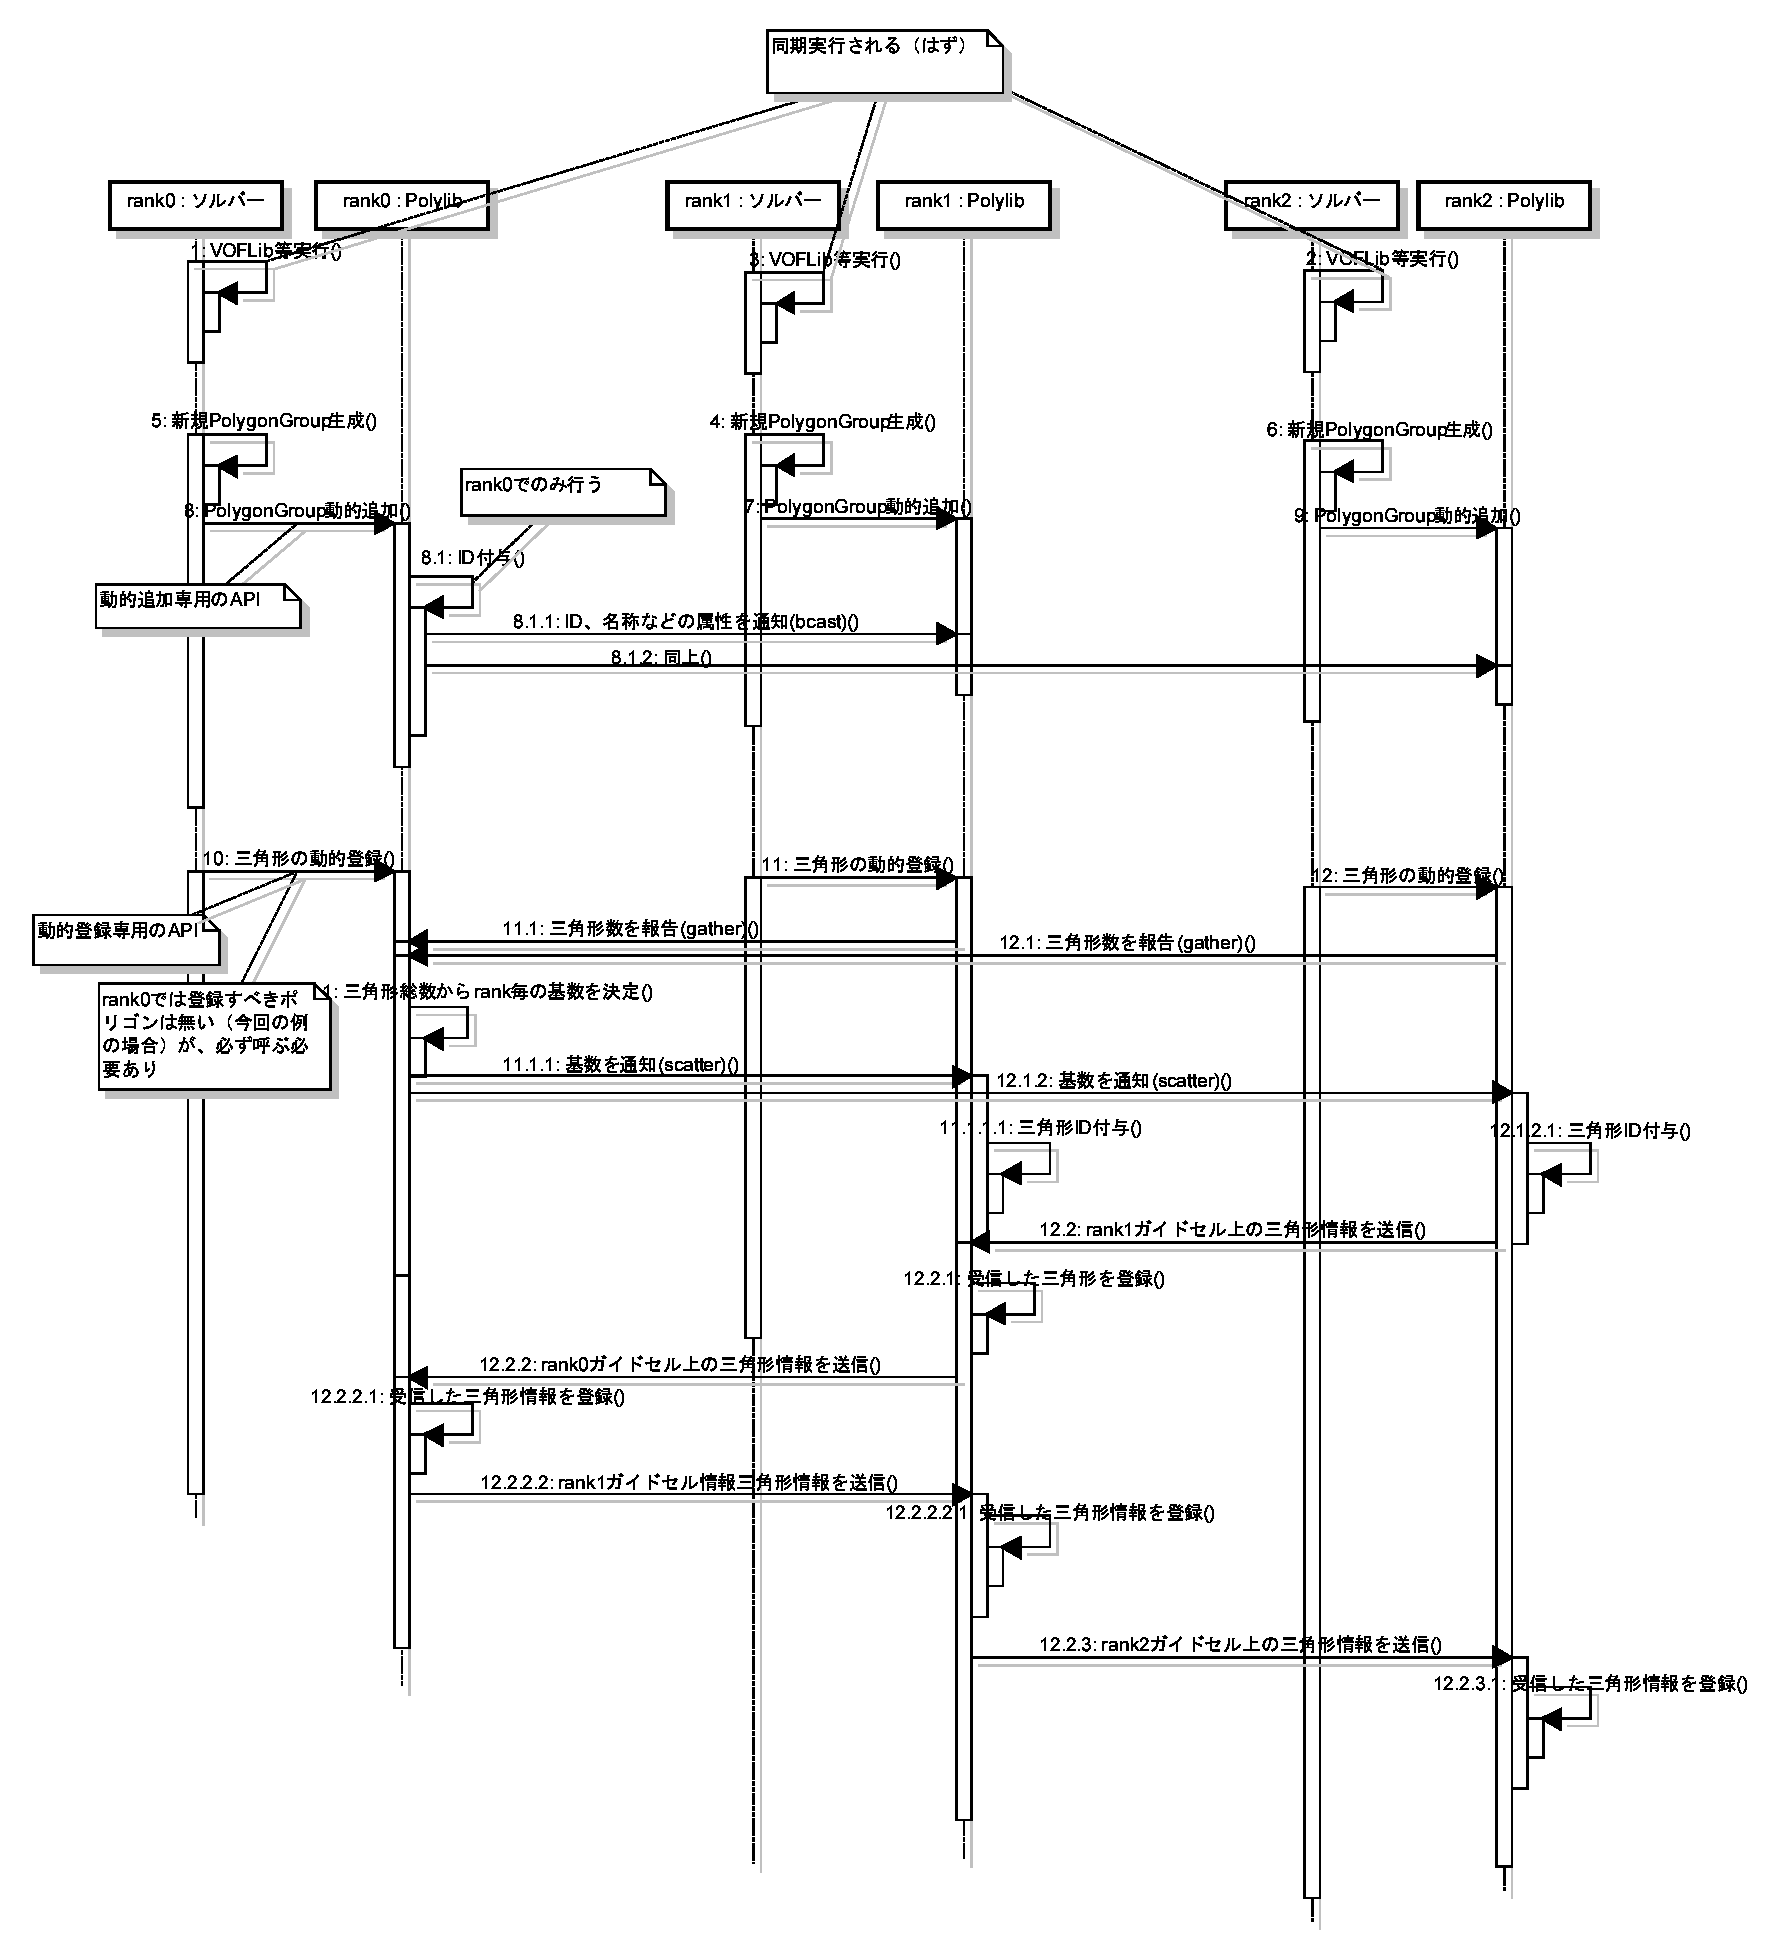
\includegraphics[width=16cm]{clip023.eps}
\end{figure}
